\documentclass[10pt,oneside,a4paper]{article}
\usepackage[IL2]{fontenc} % lepšia sadzba písmena Ľ než v T1
\usepackage[utf8]{inputenc}
\usepackage{graphicx}
\usepackage{url} % príkaz \url na formátovanie URL
\usepackage{hyperref} % odkazy v texte budú aktívne (pri niektorých triedach dokumentov spôsobuje posun textu)

\usepackage{cite}

\pagestyle{headings}
\title{Procedural Game Content Generation Using the Wave Function Collapse Algorithm\thanks{Semester project in the subject Methods of engineering work, year 2022/23, management: Name Surname}}
\author{Martin Dinja\\[2pt]
	{\small Slovak University of Technology in Bratislava}\\
	{\small Faculty of Informatics and Information Technologies}\\
	{\small \texttt{xdinja@stuba.sk}}
}

\date{\small 30.\ september 2022}

\begin{document}

\maketitle

% \tableofcontents

\begin{abstract}
    \begin{center}
        This thesis deals with the problem of generating game content using the Wave Function Collapse algorithm. The algorithm is described in detail and its application to the generation of game content is demonstrated. The thesis also contains a comparison of the algorithm with other methods of generating game content.
    \end{center}
\end{abstract}

\section{Introduction}\label{sec:introduction}

% An Introduction to the application of the wave function collapse algorithm for procedural generation of game content.
Procedural content generation (PCG) is a general term for a system that follows some patterns and generates an output based on those patterns.
Its use case is generating assets or content that would be too time-consuming to create manually.
PCG is mainly connotatively tied to game content generation, but its use cases can be more creative.
Most PCG systems use game-specific assets with game-specific rules and algorithms to generate their content.
A more general application fit for a wide range of games is the Wave Function Collapse algorithm developed by Maxim Gumin~\cite{WFC}.
Wave Function Collapse is a greedy PCG algorithm based on the concept of collapsing a wave function, which is a mathematical representation of a quantum state.
This method can generate a large, high-quality, consistent output from a small set of input patterns.
It can be used in various applications, although its most commonly used for generating 2D tilemaps for games.
It can also generate 3D models, music, poetry, and more.
WFC's output can only be as good as its input, so it's essential to have a good set of input patterns and rules. 
My goal in this thesis is to create a simple, configurable application that will use the WFC algorithm to generate tilemaps for games, given a user-defined set of input patterns and rules.

\section{Theory}\label{sec:theory}
% Theoretical background of the wave function collapse algorithm.
As mentioned in the introduction [\ref*{sec:introduction}], the Wave Function Collapse algorithm is a greedy PCG algorithm based on the concept of collapsing a wave function, which is a mathematical representation of a quantum state.
A function starts in a superposition of values and collapses when that function is measured.
The result of the measurement is the value of the function at that point.
So applying that to the PCG of a 2D tilemap, first, we need to define a set of input patterns and their rules concerning each other.
Then the algorithm will assign each tile a superposition of all possible patterns.
After prepending the superpositions, the algorithm will assign one random pattern to a tile with the least superpositions, also known as the least entropy, effectively collapsing its wave function, which is also why it is called a collapse algorithm.
Then we reevaluate all the affected tiles and their possible patterns and remove the ones that don't fit the rules.
Then we repeat the process until there is no more entropy in the tilemap.

\section{Model Implementation}\label{sec:implementation}
WFC can be divided into two models, the overlap model and the tiling model.
The overlap model is great for 2d textures, while the tiling model can be manually configured with more complex making it more suitable for game content generation.
Here we will focus on the tiling model.

\subsection{Semi-Automatic Rule System}
Rather than detailing every relation to every possible rotation of every tile. We use an array of four numbers representing a connection type for each side of the tile. \texttt{[top, right, bottom, left]}.
Only the same connection types are allowed to connect to each other.
The system than automatically generates all the possible rotations of the tile and their connections.
We can also define which tile can connect to which other tile. Making sure that for even if the connection types match, we can still prevent the tiles from connecting to each other if needed.

\begin{figure}[ht]
    \centering
    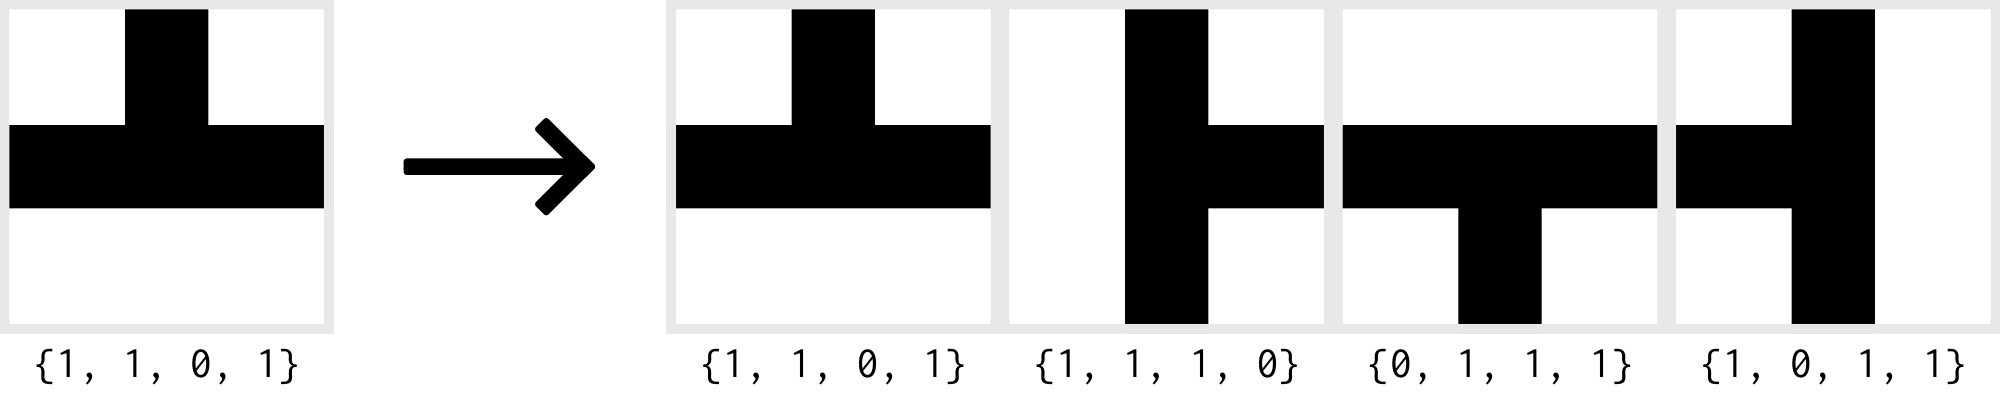
\includegraphics[width=0.8\textwidth]{figures/tile_rotation_example.png}
    \caption{Tile Rotation}\label{fig:tile_rotation_example}
\end{figure}

\subsection{Algorithm}\label{sec:algorithm}
% The main part of the project.
The central part of the project is the algorithm itself.
It uses the helper, interface, and infrastructure functions to work with the tile grid.
It starts by infering all the rules using the system mentioned in the previous section.
Then it initialize the tile grid and fill each tile's state array with all possible states.
And the the main loop of the algorithm starts.
In the loop, we get the tile with the least entropy, collapse it, and reevaluate all the affected cells.
Evaluating the cells is done by updating the states of each neighbor of the collapsed cell, then reevaluating the states of their neighbors, and so on, until we reach a point where cell states don't change any more.
Finally, we check if all of the cells are collapsed, and if they are, the algorithm halts.
Otherwise, we repeat the loop.

\begin{figure}[ht]
    \centering
    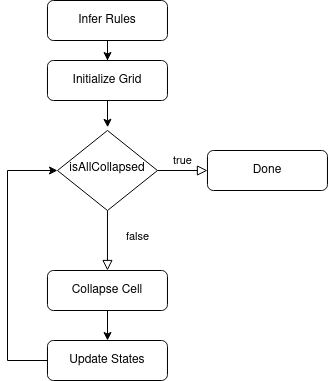
\includegraphics[width=0.6\textwidth]{figures/model_loop_diagram.png}
    \caption{Model Loop Diagram}\label{fig:model_loop_diagram}
\end{figure}

\subsection{Modifications}\label{sec:modifications}
% Modifications to the algorithm.
The algorithm is very simple and straightforward, but it can be modified to fit different needs.
For a more controlled distribution of tile types we can assign a weight value to each type.
The weight value will be used to determine the likelihood of a tile being collapsed into a certain pattern.

We can also expand WFC with generic search, giving it the ability to generate levels targeting specific play experiences.
This is the topic of a paper released by Raphael Bailly and Guillaume Levieux\cite{BL22}.

There is also a way to augment the algorithm with the Growing Grid neural network for procedural map generation~\cite{NMBP20}

We can take control to another level and introduce more constraints to the algorithm making the output seem more Human-Designed.
As detailed in the paper by Darui Cheng, Honglei Han, and Guangzheng Fei\cite{CHF20}.

And Of course there are many more ways to modify the algorithm for different purposes.

\section{Results}\label{sec:results}
% subsections: examples, performance, conclusions.
With the algorithm implemented, we can now generate tilemaps.
Starting off with a simple example (Figure~\ref{fig:example1}).
\begin{figure}[h]
    \centering
    
\includegraphics[width=0.5\textwidth]{figures/road_tiles.png}
    \caption{Road Tiles}\label{fig:example1}
\end{figure}

Defining the rules for these tiles, we can generate a 10 by 10 tilemap with the following result (Figure~\ref{fig:example1map}):
The generation shouldn't take more than a second.

\begin{figure}[h]
    \centering
    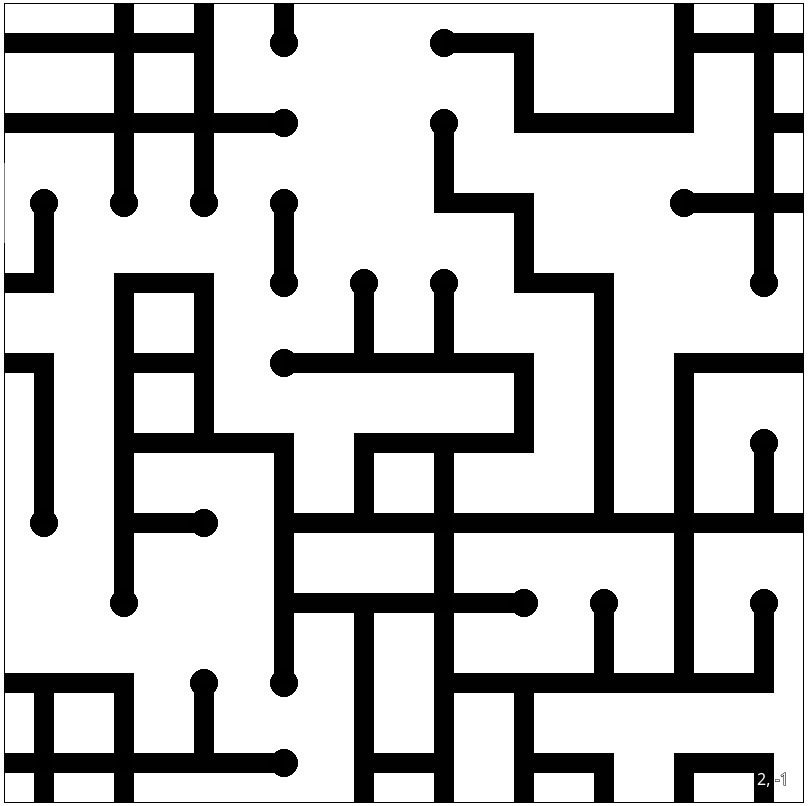
\includegraphics[width=0.5\textwidth]{figures/roads_output.png}
    \caption{Road Output}\label{fig:example1map}
\end{figure}

Altho the algorithms is very simple, it tends to break when the rule-set is more complex, and when the grid size is bigger.
This is due to the fact that the algorithm is greedy and it tends to collapse the most common patterns first, which can lead to a lot of dead-ends.

Optimizations can be made to the algorithm, and the rule system can be expanded to support more complex rules.
There is a lot of room for improvement, but for now, it is a good start.

\section{Comparison with other methods}\label{sec:comparison}
% subsections: other methods, pros and cons.
When it comes to procedurally generating some content, there are countless of other methods than WFC to choose from.
Some of them are more suited for more specific tasks, while others are more general.
Some are faster, while others are slower. Some are more complex, while others are simpler.
Comparing them is a difficult task, since they have wildly different approaches and goals.
But we can still compare WFC to some of the more related methods.

As previously mentioned WFC is a constraint-based algorithm. This makes it very configurable, and very deterministic, but it's not very interactive.
A very similar algorithm is Model Synthesis, which is a constraint-based algorithm mainly used for generating 3D models.
Paul Merrell, the creator of model synthesis has compared the two algorithms in his paper\cite{Mer21}.
\begin{quote}
    \textit{Model synthesis and WFC use nearly the same algorithm and produce similar results. WFC picks cells in a different
order and does not modify in blocks. This causes the algorithm to fail more on some large models.}
\end{quote}

Another algorithm that is very similar to WFC is the Cellular Automata algorithm.
Cellular Automata's model consists of a grid of cells, each of which has a state.
The state of a cell is determined by the state of its neighbors. Each new generation is created according to a set of rules.
The rules are usually simple, and the algorithm is very fast, but it's not very controllable or deterministic.
Its main use case is in generating terrain like caves, rivers, and mountains. It is the foundation for the world generation of Minecraft.

\begin{figure}[!h]
    \centering
    
\includegraphics[width=0.5\textwidth]{figures/cellular-automata-cave.png}
    \caption{Cellular Automata Cave Example}\label{fig:cellular_automata}
\end{figure}

\section{Conclusion}\label{sec:conclusion}
In this thesis, we had a brief introduction to PCG algorithms.
We then went over the Wave Function Collapse algorithm, and its implementation.
We explained in detail how the algorithm works, a way to implemented it, and how it can be modified.
We also showed some examples of the algorithm in action, and compared it to some other PCG algorithms.
WFC is a very simple algorithm, but it's very powerful and can be used to generate a wide variety of content.
It also has a very simple implementation, and can be easily modified to fit different needs.
It's a great algorithm to start with when learning about PCG\@.

\bibliography{lit}
\bibliographystyle{alpha}

\end{document}
